\documentclass[border=12pt]{standalone}
\usepackage{amsmath,amssymb,bm}
\usepackage{tikz}
\usetikzlibrary{positioning,arrows.meta,fit,backgrounds}
\tikzset{
  box/.style={draw, rounded corners=4pt, line width=0.8pt, inner sep=7pt, align=center, fill=white},
  stage/.style={draw, rounded corners=6pt, line width=0.8pt, inner sep=8pt},
  lab/.style={font=\bfseries\large, anchor=south west},
  arr/.style={-{Stealth[length=3mm]}, line width=1pt},
  darr/.style={-{Stealth[length=3mm]}, line width=0.8pt, dashed, gray},
}
\definecolor{cbulk}{HTML}{E3EEFB}\definecolor{cshear}{HTML}{E6F5E6}
\definecolor{ccent}{HTML}{FDF0E0}\definecolor{cchart}{HTML}{F3E6F7}\definecolor{cdata}{HTML}{F2F2F2}
\definecolor{cnote}{HTML}{FFFBE0}
\newcommand{\NN}{\mathcal{N}}
\newcommand{\re}{\operatorname{Re}}\newcommand{\im}{\operatorname{Im}}
\newcommand{\gb}{\bar g}\newcommand{\eb}{\bar e}\newcommand{\Eb}{\bar E}
\newcommand{\bnd}{\operatorname{b}}

\begin{document}
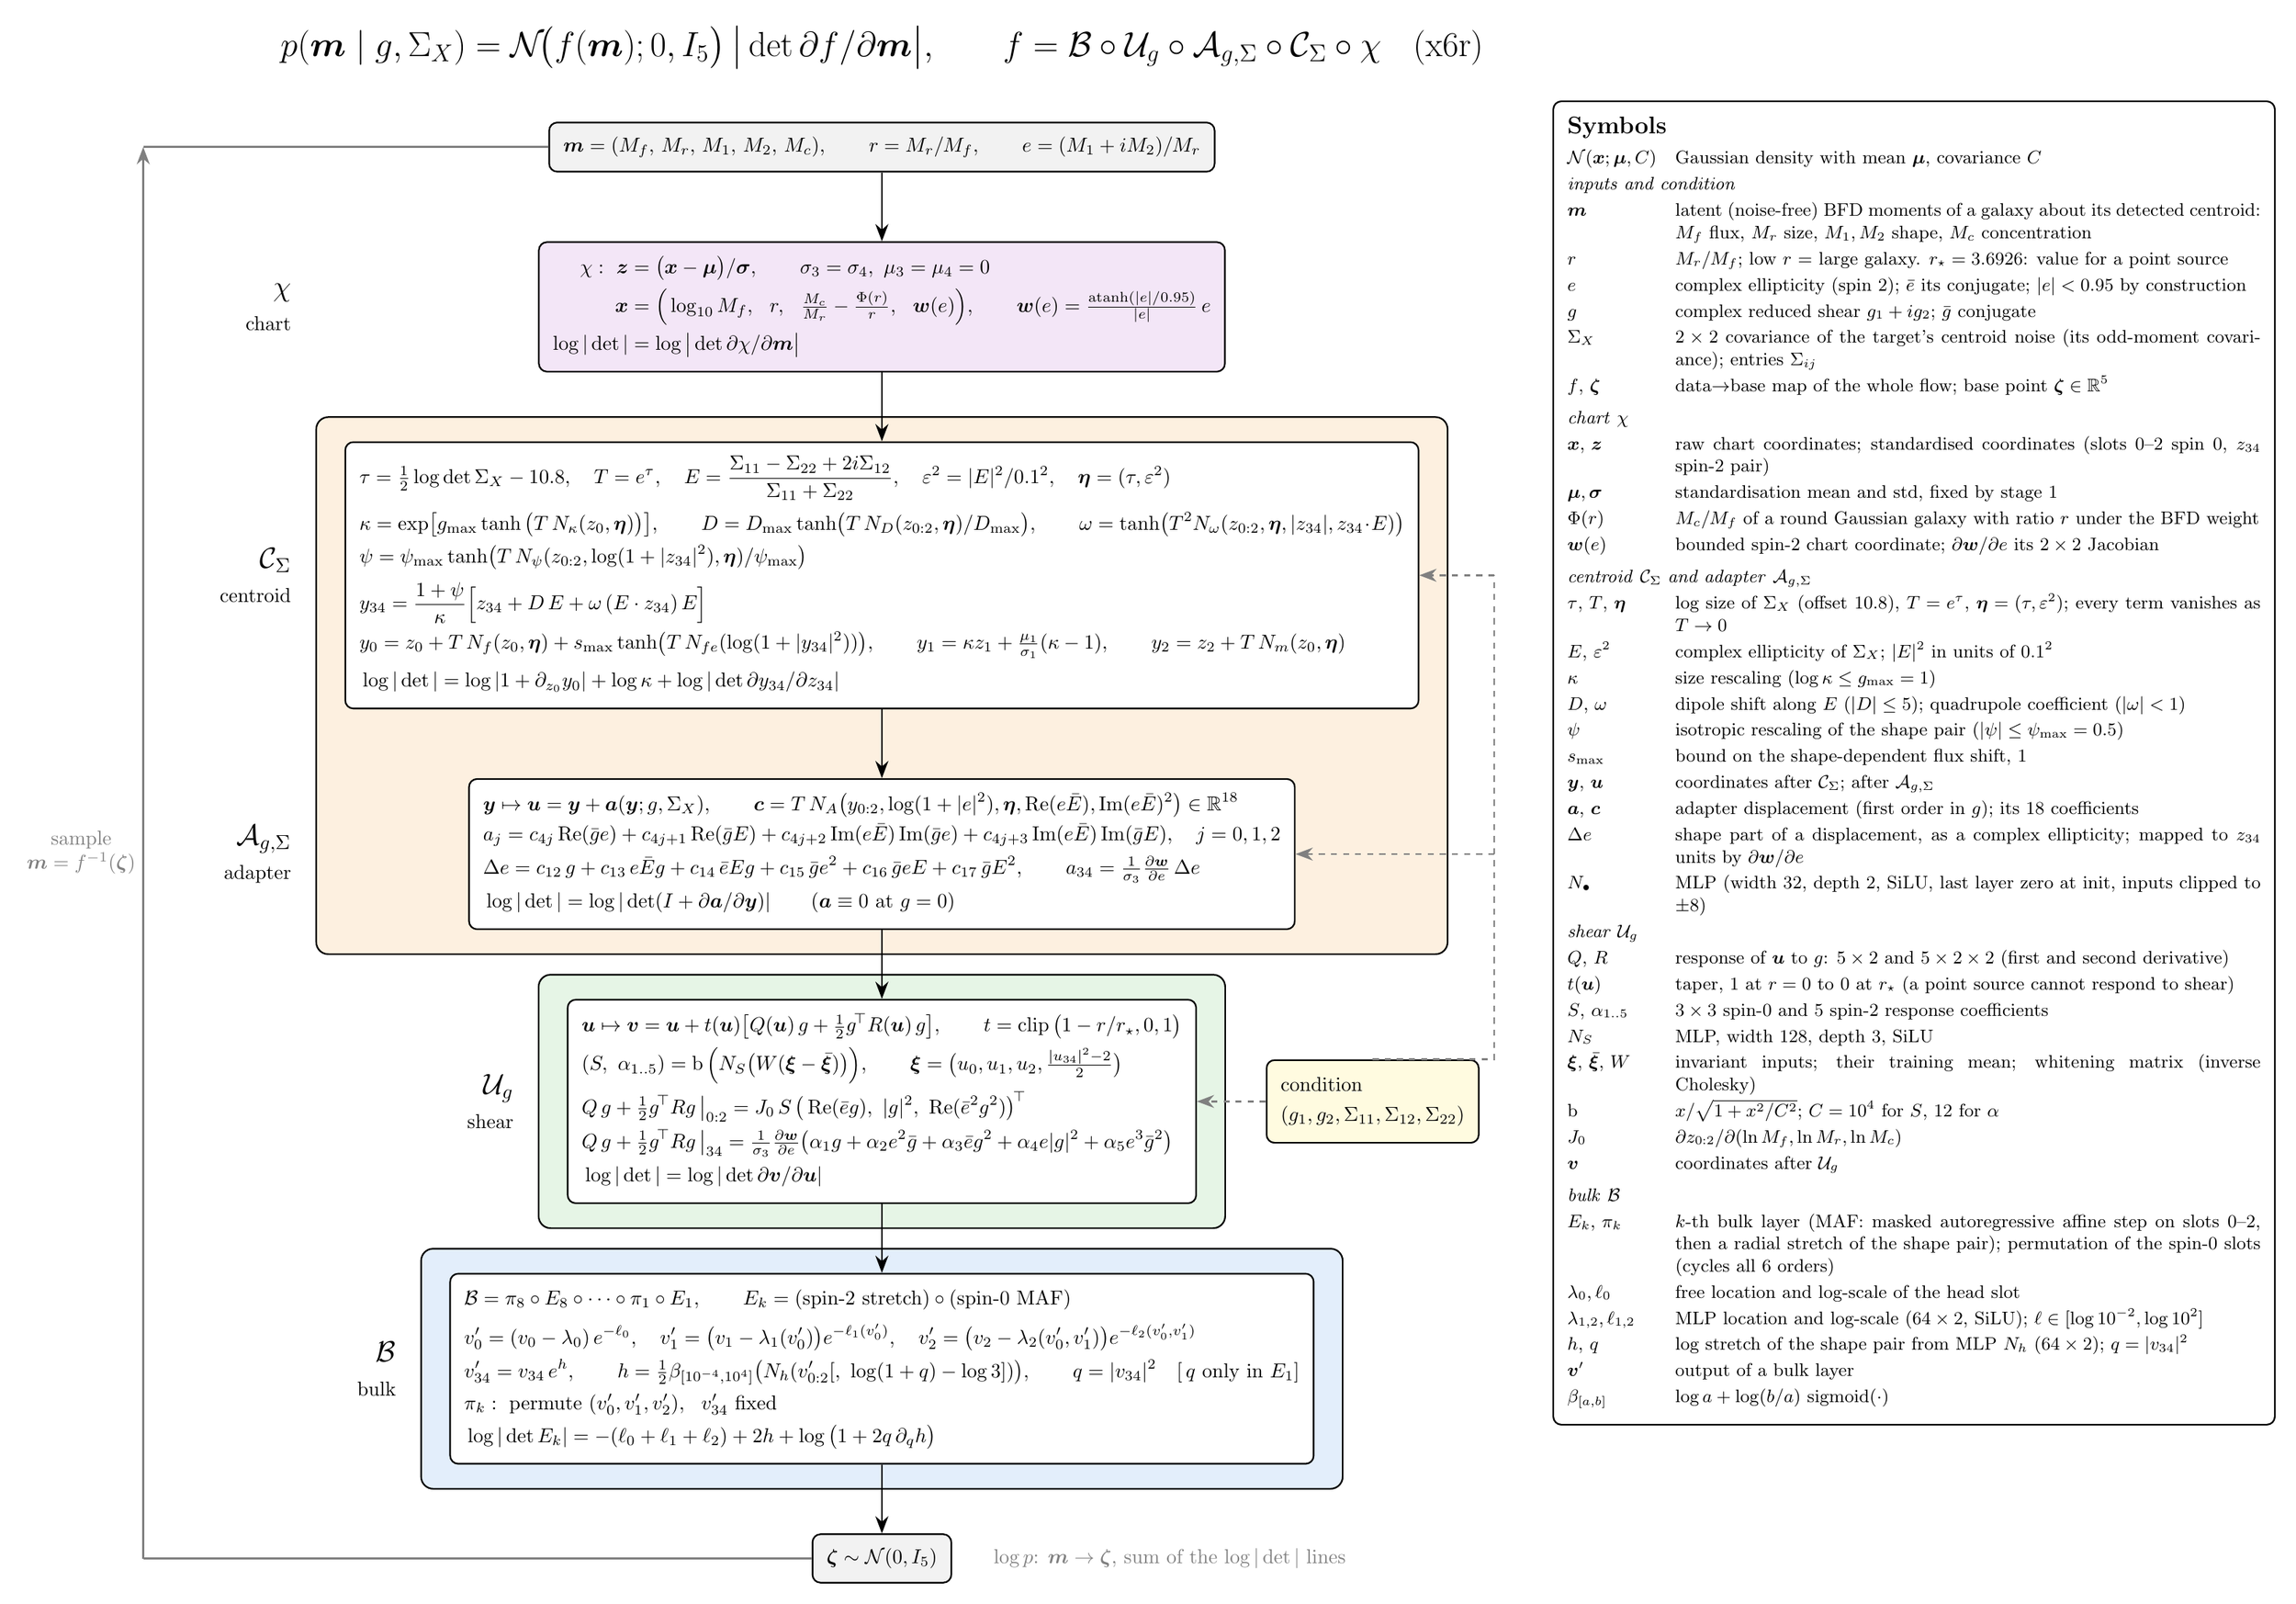
\begin{tikzpicture}[node distance=12mm]
\node[font=\LARGE] (title) {$\displaystyle p(\bm m\mid g,\Sigma_X)=\NN\!\big(f(\bm m);0,I_5\big)\,\big|\det \partial f/\partial \bm m\big|,\qquad
f=\mathcal{B}\circ\mathcal{U}_g\circ\mathcal{A}_{g,\Sigma}\circ\mathcal{C}_{\Sigma}\circ\chi$\quad (x6r)};

\node[box, fill=cdata, below=8mm of title] (m) {$\bm m=(M_f,\,M_r,\,M_1,\,M_2,\,M_c),\qquad r=M_r/M_f,\qquad e=(M_1+iM_2)/M_r$};

\node[box, fill=cchart, below=of m] (chart) {$\begin{aligned}
\chi:\ \bm z&=\big(\bm x-\bm\mu\big)/\bm\sigma,\qquad \sigma_3=\sigma_4,\ \mu_3=\mu_4=0\\
\bm x&=\Big(\log_{10}M_f,\ \ r,\ \ \tfrac{M_c}{M_r}-\tfrac{\Phi(r)}{r},\ \ \bm w(e)\Big),\qquad
\bm w(e)=\tfrac{\operatorname{atanh}(|e|/0.95)}{|e|}\,e\\
\log|\det| &= \log\big|\det\partial\chi/\partial\bm m\big|
\end{aligned}$};

\node[box, below=of chart] (sx) {$\begin{aligned}
&\tau=\tfrac12\log\det\Sigma_X-10.8,\quad T=e^{\tau},\quad E=\frac{\Sigma_{11}-\Sigma_{22}+2i\Sigma_{12}}{\Sigma_{11}+\Sigma_{22}},\quad \varepsilon^2=|E|^2/0.1^2,\quad \bm\eta=(\tau,\varepsilon^2)\\[2pt]
&\kappa=\exp\!\big[g_{\max}\tanh\big(T\,N_\kappa(z_0,\bm\eta)\big)\big],\qquad
D=D_{\max}\tanh\!\big(T\,N_D(z_{0:2},\bm\eta)/D_{\max}\big),\qquad
\omega=\tanh\!\big(T^2 N_\omega(z_{0:2},\bm\eta,|z_{34}|,z_{34}\!\cdot\!E)\big)\\
&\psi=\psi_{\max}\tanh\!\big(T\,N_\psi(z_{0:2},\log(1+|z_{34}|^2),\bm\eta)/\psi_{\max}\big)\\[2pt]
&y_{34}=\frac{1+\psi}{\kappa}\Big[z_{34}+D\,E+\omega\,(E\cdot z_{34})\,E\Big]\\
&y_0=z_0+T\,N_f(z_0,\bm\eta)+s_{\max}\tanh\!\big(T\,N_{fe}(\log(1+|y_{34}|^2))\big),\qquad
y_1=\kappa z_1+\tfrac{\mu_1}{\sigma_1}(\kappa-1),\qquad y_2=z_2+T\,N_m(z_0,\bm\eta)\\[2pt]
&\log|\det|=\log|1+\partial_{z_0}y_0|+\log\kappa+\log|\det\partial y_{34}/\partial z_{34}|
\end{aligned}$};

\node[box, below=of sx] (ad) {$\begin{aligned}
&\bm y\mapsto\bm u=\bm y+\bm a(\bm y;g,\Sigma_X),\qquad \bm c=T\,N_A\big(y_{0:2},\log(1+|e|^2),\bm\eta,\re(e\Eb),\im(e\Eb)^2\big)\in\mathbb R^{18}\\
&a_j=c_{4j}\re(\gb e)+c_{4j+1}\re(\gb E)+c_{4j+2}\im(e\Eb)\im(\gb e)+c_{4j+3}\im(e\Eb)\im(\gb E),\quad j=0,1,2\\
&\Delta e=c_{12}\,g+c_{13}\,e\Eb g+c_{14}\,\eb E g+c_{15}\,\gb e^2+c_{16}\,\gb eE+c_{17}\,\gb E^2,\qquad
a_{34}=\tfrac{1}{\sigma_3}\tfrac{\partial\bm w}{\partial e}\,\Delta e\\
&\log|\det|=\log|\det(I+\partial\bm a/\partial\bm y)|\qquad(\bm a\equiv0\ \text{at}\ g=0)
\end{aligned}$};

\node[box, below=of ad] (sh) {$\begin{aligned}
&\bm u\mapsto\bm v=\bm u+t(\bm u)\big[Q(\bm u)\,g+\tfrac12 g^{\!\top}R(\bm u)\,g\big],\qquad t=\operatorname{clip}\big(1-r/r_\star,0,1\big)\\
&(S,\ \alpha_{1..5})=\bnd\Big(N_S\big(W(\bm\xi-\bar{\bm\xi})\big)\Big),\qquad \bm\xi=\big(u_0,u_1,u_2,\tfrac{|u_{34}|^2-2}{2}\big)\\
&Q\,g+\tfrac12g^{\!\top}Rg\,\big|_{0:2}=J_0\,S\,\big(\re(\eb g),\ |g|^2,\ \re(\eb^2g^2)\big)^{\!\top}\\
&Q\,g+\tfrac12g^{\!\top}Rg\,\big|_{34}=\tfrac{1}{\sigma_3}\tfrac{\partial\bm w}{\partial e}\big(\alpha_1g+\alpha_2e^2\gb+\alpha_3\eb g^2+\alpha_4e|g|^2+\alpha_5e^3\gb^2\big)\\
&\log|\det|=\log|\det\partial\bm v/\partial\bm u|
\end{aligned}$};

\node[box, below=of sh] (bk) {$\begin{aligned}
&\mathcal B=\pi_8\circ E_8\circ\cdots\circ\pi_1\circ E_1,\qquad E_k=\text{(spin-2 stretch)}\circ\text{(spin-0 MAF)}\\[2pt]
&v'_0=(v_0-\lambda_0)\,e^{-\ell_0},\quad v'_1=\big(v_1-\lambda_1(v'_0)\big)e^{-\ell_1(v'_0)},\quad v'_2=\big(v_2-\lambda_2(v'_0,v'_1)\big)e^{-\ell_2(v'_0,v'_1)}\\
&v'_{34}=v_{34}\,e^{h},\qquad h=\tfrac12\beta_{[10^{-4},10^4]}\big(N_h(v'_{0:2}[,\ \log(1+q)-\log3])\big),\qquad q=|v_{34}|^2\quad[\,q\text{ only in }E_1]\\
&\pi_k:\ \text{permute }(v'_0,v'_1,v'_2),\ \ v'_{34}\ \text{fixed}\\
&\log|\det E_k|=-(\ell_0+\ell_1+\ell_2)+2h+\log\big(1+2q\,\partial_q h\big)
\end{aligned}$};

\node[box, fill=cdata, below=of bk] (base) {$\bm\zeta\sim\NN(0,I_5)$};

\draw[arr] (m) -- (chart);
\draw[arr] (chart) -- (sx); \draw[arr] (sx) -- (ad); \draw[arr] (ad) -- (sh); \draw[arr] (sh) -- (bk); \draw[arr] (bk) -- (base);

\begin{scope}[on background layer]
\node[stage, fill=ccent, fit=(sx)(ad), inner xsep=14pt, inner ysep=12pt] (Cc) {};
\node[stage, fill=cshear, fit=(sh), inner xsep=14pt, inner ysep=12pt] (Cs) {};
\node[stage, fill=cbulk, fit=(bk), inner xsep=14pt, inner ysep=12pt] (Cb) {};
\end{scope}
\node[font=\Large, anchor=east, align=right] at ([xshift=-3mm]sx.west -| Cc.west) {$\mathcal C_\Sigma$\\[-1pt]{\normalsize centroid}};
\node[font=\Large, anchor=east, align=right] at ([xshift=-3mm]ad.west -| Cc.west) {$\mathcal A_{g,\Sigma}$\\[-1pt]{\normalsize adapter}};
\node[font=\Large, anchor=east, align=right] at ([xshift=-3mm]Cs.west) {$\mathcal U_g$\\[-1pt]{\normalsize shear}};
\node[font=\Large, anchor=east, align=right] at ([xshift=-3mm]Cb.west) {$\mathcal B$\\[-1pt]{\normalsize bulk}};
\node[font=\Large, anchor=east, align=right] at ([xshift=-3mm]chart.west -| Cc.west) {$\chi$\\[-1pt]{\normalsize chart}};

\node[box, fill=cnote, right=12mm of sh] (cond) {$\begin{aligned}&\text{condition}\\&(g_1,g_2,\Sigma_{11},\Sigma_{12},\Sigma_{22})\end{aligned}$};
\coordinate (R) at ([xshift=8mm]Cc.east);
\draw[darr] (cond) -- (sh); \draw[gray, dashed, line width=0.8pt] (cond.north) |- (R |- cond.north) -- (R |- sx.east);
\draw[darr] (R |- ad.east) -- (ad.east); \draw[darr] (R |- sx.east) -- (sx.east);

\coordinate (L) at ([xshift=-30mm]Cc.west);
\draw[arr, gray] (L |- base) -- (L |- m) node[midway, left, align=center, text=gray]{sample\\$\bm m=f^{-1}(\bm\zeta)$};
\draw[gray, line width=1pt] (base.west) -- (L |- base); \draw[gray, line width=1pt] (L |- m) -- (m.west);
\node[right=6mm of base, text=gray, align=left] {$\log p$: $\bm m\to\bm\zeta$, sum of the $\log|\det|$ lines};

\node[box, anchor=north west, align=left, font=\small, fill=white] at ([xshift=10mm,yshift=-14mm]current bounding box.north east) {%
\renewcommand{\arraystretch}{1.18}%
\begin{tabular}{@{}l@{\quad}p{10.2cm}@{}}
\multicolumn{2}{@{}l}{\large\textbf{Symbols}}\\[2pt]
$\NN(\bm x;\bm\mu,C)$ & Gaussian density with mean $\bm\mu$, covariance $C$\\
\multicolumn{2}{@{}l}{\textit{inputs and condition}}\\
$\bm m$ & latent (noise-free) BFD moments of a galaxy about its detected centroid: $M_f$ flux, $M_r$ size, $M_1,M_2$ shape, $M_c$ concentration\\
$r$ & $M_r/M_f$; low $r$ = large galaxy. $r_\star=3.6926$: value for a point source\\
$e$ & complex ellipticity (spin 2); $\eb$ its conjugate; $|e|<0.95$ by construction\\
$g$ & complex reduced shear $g_1+ig_2$; $\gb$ conjugate\\
$\Sigma_X$ & $2\times2$ covariance of the target's centroid noise (its odd-moment covariance); entries $\Sigma_{ij}$\\
$f$, $\bm\zeta$ & data$\to$base map of the whole flow; base point $\bm\zeta\in\mathbb R^5$\\[3pt]
\multicolumn{2}{@{}l}{\textit{chart} $\chi$}\\
$\bm x$, $\bm z$ & raw chart coordinates; standardised coordinates (slots 0--2 spin 0, $z_{34}$ spin-2 pair)\\
$\bm\mu,\bm\sigma$ & standardisation mean and std, fixed by stage 1\\
$\Phi(r)$ & $M_c/M_f$ of a round Gaussian galaxy with ratio $r$ under the BFD weight\\
$\bm w(e)$ & bounded spin-2 chart coordinate; $\partial\bm w/\partial e$ its $2\times2$ Jacobian\\[3pt]
\multicolumn{2}{@{}l}{\textit{centroid} $\mathcal C_\Sigma$ \textit{and adapter} $\mathcal A_{g,\Sigma}$}\\
$\tau$, $T$, $\bm\eta$ & log size of $\Sigma_X$ (offset 10.8), $T=e^\tau$, $\bm\eta=(\tau,\varepsilon^2)$; every term vanishes as $T\to0$\\
$E$, $\varepsilon^2$ & complex ellipticity of $\Sigma_X$; $|E|^2$ in units of $0.1^2$\\
$\kappa$ & size rescaling ($\log\kappa\le g_{\max}=1$)\\
$D$, $\omega$ & dipole shift along $E$ ($|D|\le5$); quadrupole coefficient ($|\omega|<1$)\\
$\psi$ & isotropic rescaling of the shape pair ($|\psi|\le\psi_{\max}=0.5$)\\
$s_{\max}$ & bound on the shape-dependent flux shift, $1$\\
$\bm y$, $\bm u$ & coordinates after $\mathcal C_\Sigma$; after $\mathcal A_{g,\Sigma}$\\
$\bm a$, $\bm c$ & adapter displacement (first order in $g$); its 18 coefficients\\
$\Delta e$ & shape part of a displacement, as a complex ellipticity; mapped to $z_{34}$ units by $\partial\bm w/\partial e$\\
$N_\bullet$ & MLP (width 32, depth 2, SiLU, last layer zero at init, inputs clipped to $\pm8$)\\[3pt]
\multicolumn{2}{@{}l}{\textit{shear} $\mathcal U_g$}\\
$Q$, $R$ & response of $\bm u$ to $g$: $5\times2$ and $5\times2\times2$ (first and second derivative)\\
$t(\bm u)$ & taper, 1 at $r=0$ to 0 at $r_\star$ (a point source cannot respond to shear)\\
$S$, $\alpha_{1..5}$ & $3\times3$ spin-0 and 5 spin-2 response coefficients\\
$N_S$ & MLP, width 128, depth 3, SiLU\\
$\bm\xi$, $\bar{\bm\xi}$, $W$ & invariant inputs; their training mean; whitening matrix (inverse Cholesky)\\
$\bnd$ & $x/\sqrt{1+x^2/C^2}$; $C=10^4$ for $S$, $12$ for $\alpha$\\
$J_0$ & $\partial z_{0:2}/\partial(\ln M_f,\ln M_r,\ln M_c)$\\
$\bm v$ & coordinates after $\mathcal U_g$\\[3pt]
\multicolumn{2}{@{}l}{\textit{bulk} $\mathcal B$}\\
$E_k$, $\pi_k$ & $k$-th bulk layer (MAF: masked autoregressive affine step on slots 0--2, then a radial stretch of the shape pair); permutation of the spin-0 slots (cycles all 6 orders)\\
$\lambda_0,\ell_0$ & free location and log-scale of the head slot\\
$\lambda_{1,2},\ell_{1,2}$ & MLP location and log-scale ($64\times2$, SiLU); $\ell\in[\log10^{-2},\log10^{2}]$\\
$h$, $q$ & log stretch of the shape pair from MLP $N_h$ ($64\times2$); $q=|v_{34}|^2$\\
$\bm v'$ & output of a bulk layer\\
$\beta_{[a,b]}$ & $\log a+\log(b/a)\,\operatorname{sigmoid}(\cdot)$\\
\end{tabular}};
\end{tikzpicture}
\end{document}
